
\title{The Length Estimation Challenge}
\author{
        Jesika H Haria \\
                6.804J/9.660J Fall 2012 Final Project\\
	jesika@mit.edu
}
\date{\today}

\documentclass[12pt]{article}
\usepackage{amsmath,mathtools,hyperref}
\begin{document}
\maketitle

\begin{abstract}
This report investigates estimated distance perception in humans by conducting an experiment that requires subjects to estimate the length of a line as multiple of a given a reference line measurement. This was implemented in the form of a game. The time pressure of one minute to solve as many possible estimation problems, and get the highest score, effectively introduced the tradeoff of accuracy and speed,  with the hope of inducing the estimation from real-world, constraint-dominated scenarios. Results indicate that the distribution retains it aggregate shape, and each multiple of the reference line tested seemed to follow a Gaussian distribution in terms of human estimates of that multiple. This experiment was illustrative in verifying intuitive models of human estimation. 
\end{abstract}

\section{Introduction}\label{introduction}
Estimation is a key concept in learning, especially for most of the spatial, reasoning and mathematical skills used in daily life. Estimating distance between places, estimating the number of items that will fit in a grocery bag, estimating how much time you have to cross a road before the red signal are some examples of situations where we use the power of estimation to guide our decisions. 
\\ \\
In this investigation, I set out to study the impact of different parameters on arbitrary length estimation, given a unit reference lengths. The parameters varied were the closeness of the reference length to the actual line whose length was to be estimated, the start point of the measurement line to the reference line, and the relative length of the reference line to the line to be measured. The goal of the game was to maximize the score, which depended on both speed and accuracy, introducing a potential trade-off.   

\section{Experimental Setup}\label{experimental setup}
\subsection{Story Outline}
This is the story that was given to the subjects prior to the experiment: 
\\\\
\textit{
Your task is to maximize your score estimating the length of the gray line, given the red line as a reference for length. You will be given different lengths of red and gray lines, and their positions on the board might vary. 
\\\\Your timer will start ticking when you press Start. Type your estimate in the text box, and hit Enter to submit. You will be notified of the right answer, then hit Next to get the next problem. 
\\\\You have one minute to complete this task, and your score will depend on the number of problems you solve as well as your accuracy solving each of them. Good luck! 
}
\subsection{Setup}
After reading the story, the subjects were presented with the following game setup \\
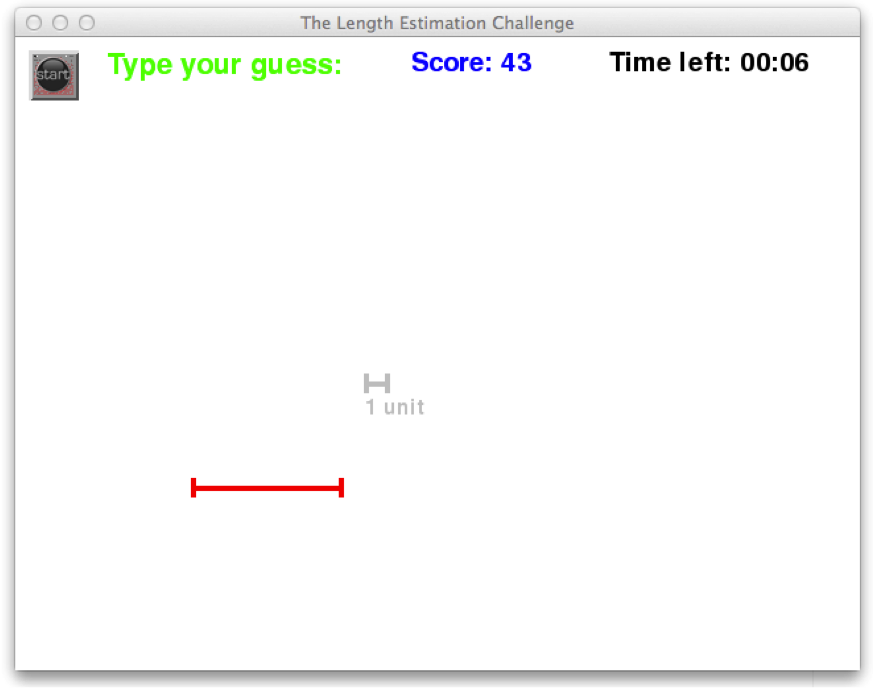
\includegraphics{/Users/jesika/Pictures/ScreenShotGame.png}
\subsection{Parameters}
The parameters chosen were: 
\begin{enumerate}
\item \emph{Distance of measurement line (red) from reference line (gray)} 
\\ The values for $d$, as measured by the distance between the leftmost point on the lines, that were tested were $50,100,150,200,250,300$ pixels. 
\item \emph{The relative length of the measurement line and the reference line}
\\ The values for $m$, as measured by the ratio of the measurement line to the reference line, was an integer between $2, 3, 4, 5, 6, 7$.  
\end{enumerate}
One reading of every combination of the two variables $d$ and $m$ was taken per subject, although the time pressure meant that some subjects did not get around to completing all 36 scenarios. 
\\\\NB: The intention behind varying the distance uniformly was to verify the correctness of the estimation for different environment scenarios, and give validity to the guess. It was also done so as to take into account that different subjects might have a different optimum distance for comparison, and the experiment must be fair in ensuring that all these distances are thus covered. 
\subsection{Source}
The game was made using PyGame, which is a Python library for making games, and the source code can be found on GitHub at \url{https://github.com/jharia/length-estimation-pygame}.  

\section{Hypothesis}\label{hypothesis}
Gideon Rosenblatt has previously conducted a 'Wisdom of the crowds' experiment on Google Plus, where he asked people to estimate the number of cereals in an oddly-shaped vase \cite{online experiment}. Although most people's guesses were off, the collective guess of the group was close to average. A similar situation might ensue in this experiment; while people might make mistakes in guessing, the collective distribution of their score might have a mean similar to the actual multiplier.  With some more rigor, we might posit: 
\\\\The law of large numbers (LLN) states that with sufficiently large number of examples $n$, where $n\to\infty$, the sample average $\bar{X_n}$ converges to the expected value $\mu$. In this experiment, there were a total of 727 data points, and since the order in which they were picked was random, there were approximately 120 samples per value of $m$. Let's call the average guesstimate of the subjects for a particular $m$, $g$. According to LLN, as $n\to\infty$, $g \to m$.
\\\\Furthermore, one might imagine that the actual distribution of these guesses for a particular multiplier might have the highest frequency \emph{at} the right multiplier, but some non-zero frequency for multiplier values close to it, the frequency tapering as one moves away from the original value. Let us assume this form to be Gaussian, from the Central Limit Theorem. 

\section{Observations}\label{observations}
We found that the average of the estimates for a particular multiplier, $g_i$ was close to the actual multiplier length $m_i$, for $i \in [2,3,4,5,6,7]$, but not exact, since the number of samples was limited.
\begin{figure}[!ht]
  \centering
    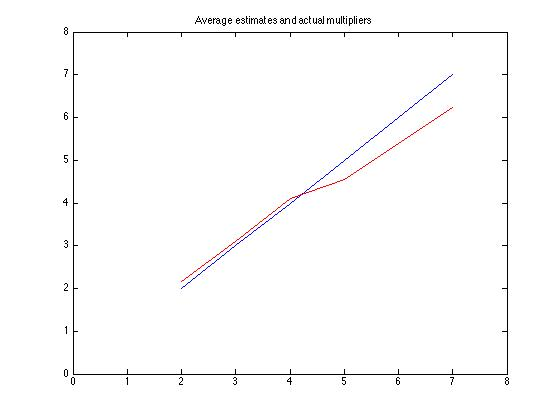
\includegraphics[width=150 mm]{/Users/jesika/Pictures/6.804/gvsm.jpg}
  \caption{Averages and estimates for different values of the multipliers}
  \label{gvsm}
\end{figure}
\\Figure~\ref{gvsm} demonstrates the averages plotted alongside the estimates. 
The relationship between the average guess and the value of the multiplier is interesting. A number of observations are thus in order. 
\\\\First, we can see that the average guess for smaller multipliers, i.e. for $m_i$s where $i \leq 4$, is higher than the value of the multiplier itself, whereas the average guess for higher multipliers, i.e. for $m_i$, where $i > 4$, is smaller than the value of the multiplier itself. We can round down the pivot point, as seen from Figure~\ref{gvsm}, to 4. 
\\\\Second, the further the multipliers are from this pivot number 4, the more inaccurate the average guess is. 
\\\\Third, the average guess is fairly accurate to the real multiplier, even with a small number of samples. The certainty of these guesses decreases as the multiplier value increases. 
\section{Discussion}\label{discussion}
\subsection{Average guess vs multiplier value}\label{average}
Let us understand the observations further. The average guess being higher for small multipliers and smaller for high multipliers seems to lend to the conclusion that people might favor a "middle" ground number, for fear of estimating too much on the extremes. The subjects were only told that the multiplier would be a single digit integer, and although the multipliers were only between 2 and 7, there was no one who guessed 9 or 1. This further ratifies the theory that medium numbers are considered less extreme, and hence a safer bet. 	
\begin{figure}[!ht]
  \centering
    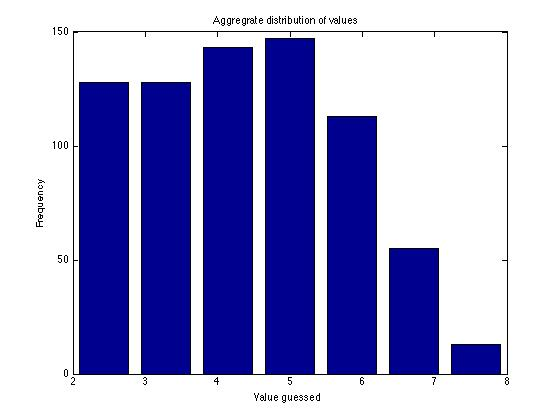
\includegraphics[width=150 mm]{/Users/jesika/Pictures/6.804/mallalt.jpg}
  \caption{Aggregate Frequency Distribution}
  \label{mallalt}
\end{figure} \\
\\Another way of ratifying this information is by observing that, for a uniform random distribution of numbers between 2 and 7, each taken 121 times, the mean is 4.5, with a variance of 2.92. In practice, with the 727 samples collected, the mean of the multipliers presented was 4.51, with variance 2.95. This randomization is a close approximation to the uniform density obtained from cycling through the choices, and helps to maintain the element of surprise in the game. The mean of the estimates was 4.26, with the variance being 2.61. This makes the estimated distribution slightly skewed towards lower guesses, which might be a result of people not wanting to overestimate, and the mean is actually strikingly close to the true pivot value we saw in Figure~\ref{gvsm}. The variance observed is lower than the theoretical variance, which confirms our model's belief that people are less likely to guess on values far away from this pivot. All the characteristics described can be found in Figure~\ref{mallalt}. Overall, the distribution seems uniform, similar to the distribution it was drawn from, with the exception at $i=7$, which is significantly lower frequency than expected. This might be because we have another value in the sample distribution, 8, that was not in the original distribution, and the frequency count of 7, which is the closest to 8 in terms of an estimate, thus suffers. Furthermore, the distributions of 4 and 5 seem to be higher than the expected frequency, further contributing to the paucity of guess of 8. The higher-than-expected frequencies of multipliers 4 and 5 ratify that these numbers were preferred over either extreme. 
\subsection{Accuracy of estimation}
Our second observation was that the further the multipliers are from the pivot point, the higher the inaccuracy of human's estimation, which can be seen in the average guess of the estimate. We might need to dig one level deeper to understand why this is so. A potential reason could be because of higher uncertainty of distance perception for longer distances, a variable that can be captured by the variance of the guesses. With higher uncertainty, we might expect higher chances of error. 
\begin{table}[ht]
\caption{Mean and variance of guess} % title of Table
\centering  % used for centering table
\begin{tabular}{c c c} % centered columns (4 columns)
\hline\hline                        %inserts double horizontal lines
Actual Multiplier & Mean of Guess  & Variance of Guess \\ [0.5ex] % inserts table 
%heading
\hline                  % inserts single horizontal line
2 & 2.16 & 0.37  \\ % inserting body of the table
3 & 3.10 & 0.45\\
4 & 4.11 & 0.61\\
5 & 4.56 & 0.76\\
6 & 5.38 & 1.05 \\ 
7 & 6.22 & 1.19 \\ [1ex]      % [1ex] adds vertical space
\hline %inserts single line
\end{tabular}
\label{mvg} % is used to refer this table in the text
\end{table}

\begin{figure}[!ht]
  \centering
    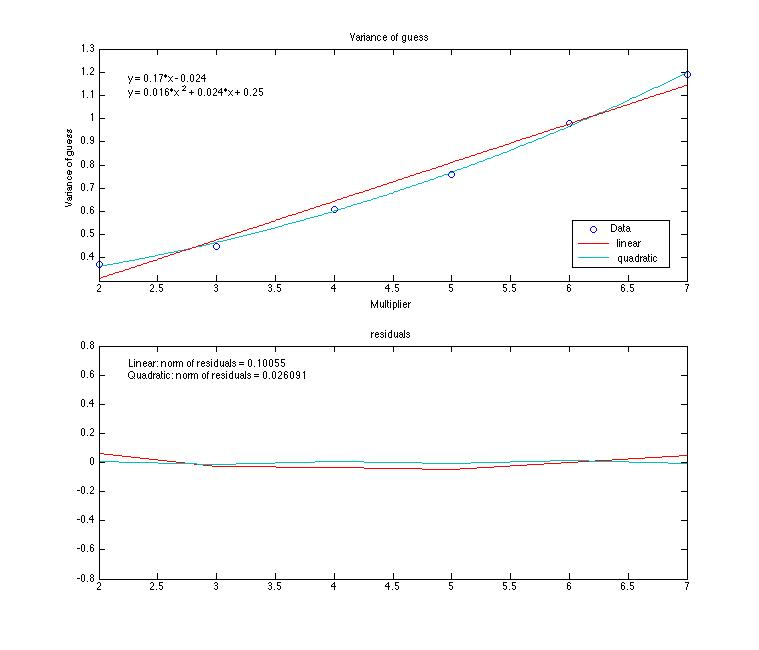
\includegraphics[width=150 mm]{/Users/jesika/Pictures/6.804/varres.jpg}
  \caption{Variances for different multipliers}
  \label{varres}
\end{figure} 
Table~\ref{mvg} reaffirms our postulation that the longer the distance, the greater the uncertainty in measurement, as measured by the variance. 
\\\\Figure~\ref{varres} demonstrates that the variance increases with increasing value of multipliers, confirming that uncertainty associated with such estimations is generally higher. In modeling an appropriate fit, both linear and quadratic curve fitting was considered. it was found that that the norm of the quadratic equation was 0.02, as opposed to that of the linear curve, which was 0.1. Using the Occam's razor approach, the quadratic model was broad enough to withstand cross-validation and not over fit, while lower order polynomials like a linear curve did not fit the data well. Hence, the quadratic model was selected. The fact that the variance is the square of the difference between the mean and the sample value might also support the quadratic increase in the variance with increasing multipliers. 
\subsection{Distribution of the guess: mean and variance}
Our third observation was that the average guess was fairly close to the actual multiplier, as was reflected in Figure~\ref{gvsm}. We might want to investigate the frequency distribution of this guess further in order to determine a more accurate model for human estimation. 
\begin{figure}[!ht]
  \centering
    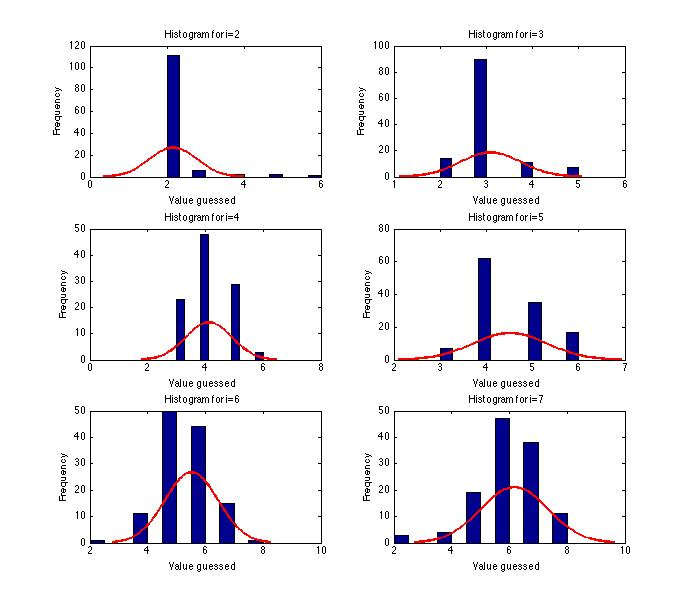
\includegraphics[width=150 mm]{/Users/jesika/Pictures/6.804/allm.jpg}
  \caption{Frequency distribution for different multipliers}
  \label{allm}
\end{figure} \\
Figure~\ref{allm} shows how the frequency distribution changes with the $i$ being tested. We model this as a Gaussian, to illustrate the fact that as you move away from the average, the frequency drastically drops. Some of the $i$s towards the end points, notably $i=2$ have skewed distributions because subjects didn't rate a 0 or 1 on any line. The skew in each graph also serves to steer the mean of the Gaussian away from the true multiplier value, and has been discussed in Section~\ref{average}. The plots also clearly illustrate that for lower multipliers, the skew tends to be towards values greater than the actual mean, and for higher multipliers, the skew is towards values lesser than the actual mean. This is good confirmation of our first observation from Section~\ref{observations}. 

\section{Conclusion}\label{conclusion}
The goal of this experiment was to model a part of the human distance estimation process under competing constraints. 
\\\\The results confirmed the hypothesis of the average guess converging to the actual multiplier value, with the distribution being modeled by a Gaussian with the mean close to this actual multiplier value, and a variance that is a quadratically increasing function of the actual multiplier. 
\\\\Thus, we see that human distance perception, even under pressure, performs reasonably well, with the highest probability of selecting the actual distance, within an error range that tends to 0 with increasing sample size. 

\section{Further Work}\label{further work}
There are a series of natural extensions to this experiment, the most notable one being conducting the same experiment with different parameters. For example, investigating whether the distance of the two lines changes the accuracy of the estimate, whether the relative start position of the two lines affects the ability to measure (aligned vs non-aligned), and whether the orientation of the line matters to the estimate. 
\\\\Another interesting area to explore would be other types of lines, for example, curves or random squiggles, which would no doubt be harder to estimate. This idea could be extended to estimating area, volume, number of dots in a given space, and the like. 
\\\\The game could be changed to include multi-players, which changes the dynamics by introducing direct competition. This would serve to change the scoring function. 

\bibliographystyle{abbrv}
\bibliography{main}

\begin{thebibliography}{10}
\bibitem{online experiment} Gideon Rosenblatt, \emph{Testing the Wisdom of Crowds}, April 20, 2012. \texttt{http://www.alchemyofchange.net/crowd-wisdom-test/}. Last accessed: December 15, 2012. 

\end{thebibliography}
\end{document}
This is never printed